\documentclass[a4paper]{article}
\usepackage{float}

\usepackage{amsmath}
\usepackage{amssymb}
\usepackage{graphicx}
\usepackage{inputenc}
\usepackage{hyperref}
\usepackage{listings}
\usepackage{polski}

\title{Raport}
\author{Łukasz Fabia}
\date{20.05.2024}

\begin{document}

\maketitle
\tableofcontents

\section{Wstęp}

\quad Celem badań jest analiza danych dotyczących ofert pracy w IT. W swojej pracy postaram się
odpowiedzieć na pytanie, jakie są najbardziej poszukiwane umiejętności w branży IT oraz ile można zarobić
znając dane języki, frameworki czy narzędzia. W tym celu postram się wykorzystać sci-kit learn do stworzenia
modelu regresji liniowej, który pozwoli mi przewidzieć zarobki na podstawie umiejętności (technologii).


\section{Dane}

\quad Dane pozyskam z serwisu \href{https://justjoin.it/}{justjoin.it}, który zbiera oferty pracy z wielu różnych serwisów, zatem
ofert pracy będzie całkiem sporo. Na stronie mamy katergorie, które mogą być przydatne do analizy, takie jak:
JS, PHP, Ruby, Python, Java, Net, Mobile, C, DevOps, Security, Data, Go, Game, Scala. W mojej analizie skupię się na nich.
\quad Dodatkowo analizuję zarobki tylko na b2b oraz na umowie o prace (uop), ponieważ są to najbardziej popularne formy zatrudnienia w IT a inne formy takie jak umowa
o zlecenie czy umowa o staż pratykcznie nie występują. Do analizy będę również brał pod uwagę lokalizację.

\textbf{\newline Technologia} - język programowania, framework, narzędzie, które jest wymagane w ofercie pracy.

\subsection{Model danej}
\quad Dane będą zawierały informacje o ofertach pracy, takie jak:
\begin{itemize}
    \item tytuł oferty
    \item widełki dla B2B
    \item widełki dla UOP
    \item technologie dotyczące umowy
    \item lokalizacja
    \item doświadczenie {junior, mid, senior}
    \item typ pracy {stacjonarnie, hybrydowo, zdalnie}
\end{itemize}

\subsection{Obsługa technologii, lokalizacji}

\quad Najpierw zdefiniuje sobie słownik klucz, wartość, gdzie klucz to ustandaryzowana technologia, a wartość do synonimy tej technologii.

\textit{np. \ "JavaScript": [
"javascript",
"js",
"node.js",
"nodejs",
"express.js",
"expressjs",
],}

\quad Dzięki temu będę mógł przekonwertować technologie z oferty pracy na wektor binarny, gdzie 1 oznacza, że technologia jest wymagana, a 0, że nie jest wymagana. Kolejnym
krokiem będzie obsługa lokalizacji. W tym przypadku jeśli oferta dot. kilku miast to znaczy, że pojawi się w zbiorze
klika ofert z tymi samymi danymi, ale dla różnych miast.


\subsection{Pozykiwanie danych}

\quad Dane będą pozyskiwane z ww. serwisu, za pomocą narzędzi do web scrappingu w moim przypadku będzie
to \texttt{Selenium}, ponieważ strona ma dynamicznie ładowany content.


Kroki:
\begin{itemize}
    \item napisanie skryptu pobierającego linki do ofert pracy z danej kategorii, ponieważ nie chcemy śmiecowych ofert typu Product manager
    \item napisanie skryptu przetwarzającego linki do ofert pracy, aby pobrać dane z oferty
    \item przekierowanie wyniku do pliku json.
    \item normalizacja oraz oczyszczanie danych, kodowanie technologii, do wektora przy pomocy MultiLabelBinarizer z \texttt{sklearn}
    \item kodowanie duplkacja ofert z różnymi lokalizacjami oraz kodowanie typu pracy i doświadczenia (\texttt{label encoding})
    \item usunięcie ofert z wynagrodzniem godzinowym bo zalezą one od ilości przepracowanych godzin
\end{itemize}

\textit{Ofert ze stawką godzinową było kilka więc nie wypływają one na wyniki.}

\section{Wygląd do danych}

\textit{uwaga przykładowe dane nie zawierają wszystkich kolumn bo jest ich za dużo, wszystkie dane można znaleźć w ../data/jobs.csv}


\textbf{Przykładowe dane:}


\begin{table}[h]
    \centering
    \begin{tabular}{|c|c|c|c|c|}
        \hline
        \multicolumn{1}{|c|}{\textbf{title}} & \textbf{min\_b2b} & \textbf{max\_b2b} & \textbf{min\_uop} & \textbf{max\_uop} \\ \hline
        Senior Software Engineer             & 0.0               & 0.0               & 18000.0           & 28000.0           \\ \hline
        Senior Backend Node.js Engineer      & 0.0               & 0.0               & 18360.0           & 25125.0           \\ \hline
        Senior Fullstack Developer           & 22680.0           & 27216.0           & 16600.0           & 19920.0           \\ \hline
    \end{tabular}
\end{table}


\begin{table}[h]
    \centering
    \begin{tabular}{|c|c|c|c|}
        \hline
        \textbf{location\_code} & \textbf{operating\_mode\_code} & \textbf{experience\_code} \\ \hline
        38                      & 0                              & 2                         \\ \hline
        17                      & 2                              & 2                         \\ \hline
        51                      & 0                              & 2                         \\ \hline
    \end{tabular}
\end{table}


\begin{table}[h]
    \centering
    \begin{tabular}{|c|c|c|c|}
        \hline
        \textbf{AWS} & \textbf{JavaScript} & \textbf{React} & \textbf{Java} \\ \hline
        1            & 1                   & 1              & 0             \\ \hline
        0            & 1                   & 1              & 0             \\ \hline
        1            & 1                   & 1              & 0             \\ \hline
    \end{tabular}
\end{table}

\newpage

\section{Rozkłady i statystyki}

\quad Aktualnie w zbiorze \textit{jobs.csv} znajduje się \textbf{4574} ofert pracy, które będą poddane
analizie. Wszystkie dane są znormalizowane i gotowe do analizy. Analizę można zacząć od średniej zarobków
dla kontraktu B2B oraz UOP.


\textbf{Widełki dla Juniora: }

\begin{table}[h]
    \centering
    \begin{tabular}{|c|c|c|c|}
        \hline
        \textbf{PLN}             & \textbf{B2B} & \textbf{UOP} \\ \hline
        \textbf{średnie widełki} & 8555.40      & 13558.71     \\ \hline
        \textbf{min widełki}     & 4250.00      & 6000.00      \\ \hline
        \textbf{max widełki}     & 16443.00     & 28000.00     \\ \hline
    \end{tabular}
    \caption{Średnie zarobki w PLN dla \texttt{juniora} w Polsce}
\end{table}

\textbf{Widełki dla Mida: }

\begin{table}[h]
    \centering
    \begin{tabular}{|c|c|c|c|}
        \hline
        \textbf{PLN}             & \textbf{B2B} & \textbf{UOP} \\ \hline
        \textbf{średnie widełki} & 12378.99     & 18041.77     \\ \hline
        \textbf{min widełki}     & 5000.00      & 7000.00      \\ \hline
        \textbf{max widełki}     & 25000.00     & 30000.00     \\ \hline
    \end{tabular}
    \caption{Średnie zarobki w PLN dla \texttt{mida} w Polsce}
\end{table}

\textbf{Widełki dla Seniora: }

\begin{table}[h]
    \centering
    \begin{tabular}{|c|c|c|c|}
        \hline
        \textbf{PLN}             & \textbf{B2B} & \textbf{UOP} \\ \hline
        \textbf{średnie widełki} & 18930.61     & 25848.46     \\ \hline
        \textbf{min widełki}     & 8000.00      & 11000.00     \\ \hline
        \textbf{max widełki}     & 40000.00     & 80000.00     \\ \hline
    \end{tabular}
    \caption{Średnie zarobki w PLN dla \texttt{seniora} w Polsce}
\end{table}
\newpage
\subsection{Jak się pracuje w IT?}

\begin{figure}[H]
    \centering
    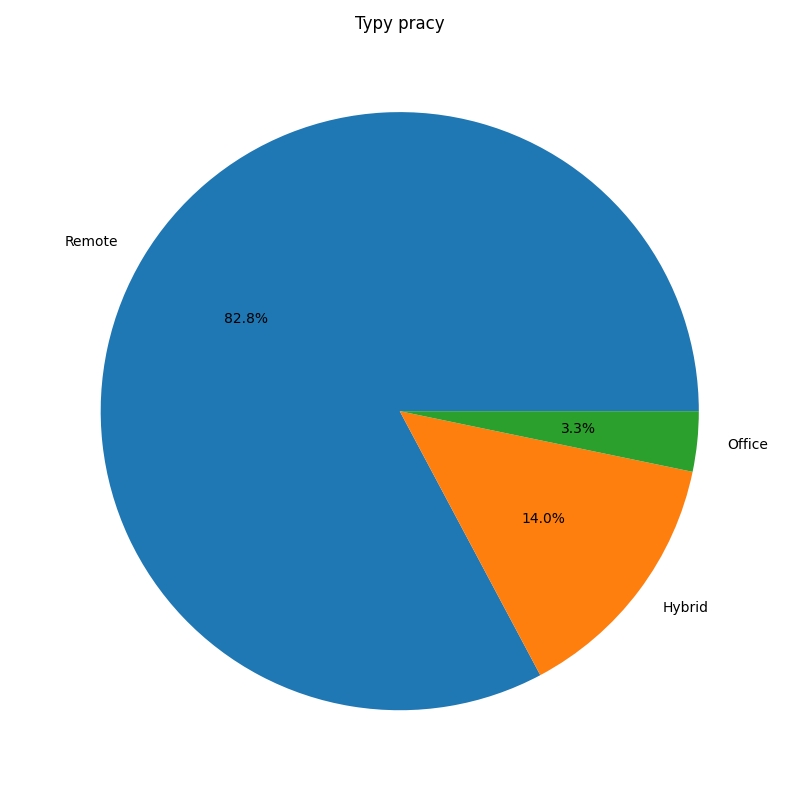
\includegraphics[width=0.8\textwidth]{../analysis/plots/rozkłady/typy_pracy.png}
    \caption{Rozkład typów pracy}
\end{figure}

\quad Jak widać najwięcej ofert pracy dotyczy pracy zdalnej.


\subsection{Kogo szukają pracodawcy?}

\begin{figure}[H]
    \centering
    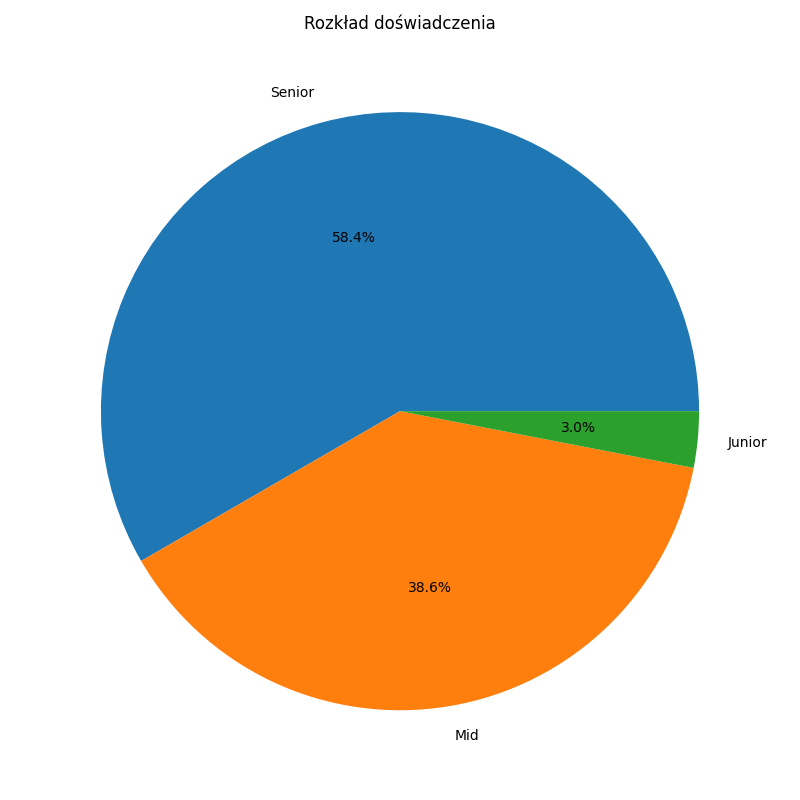
\includegraphics[width=0.8\textwidth]{../analysis/plots/rozkłady/rozkład_doświadczenia.png}
    \caption{Rozkład typów pracy}
\end{figure}

\quad Tak jak można było się spodziewać - najwięcej ofert pracy jest dla seniorów,
stąd też wynika dlaczego tak dużo kontraktów dotyczy pracy zdalnej. Chociaż
warto powiedzieć sytuacja midów jest również dobra. Gorzej jest z ofertami dla młodych programistów.
Tutaj liczba ofert wyniosła zaledwie 139, co jest bardzo małą liczbą w porównaniu do innych grup.

\textit{Czy to oznacza, że młodzi programiści mają trudniej, a słynne "eldorado" w IT jest tylko dla doświadczonych programistów?}

\quad Tutaj można powiedzieć, że juniorzy mają trudniej \textbf{wejść} do branży, ale zarobki po wejściu są naprawdę atrakcyjne,
no, ale tutaj problem może być z wejściem.


\subsection{Jak rozkładają się zarobki?}

\begin{figure}[H]
    \centering
    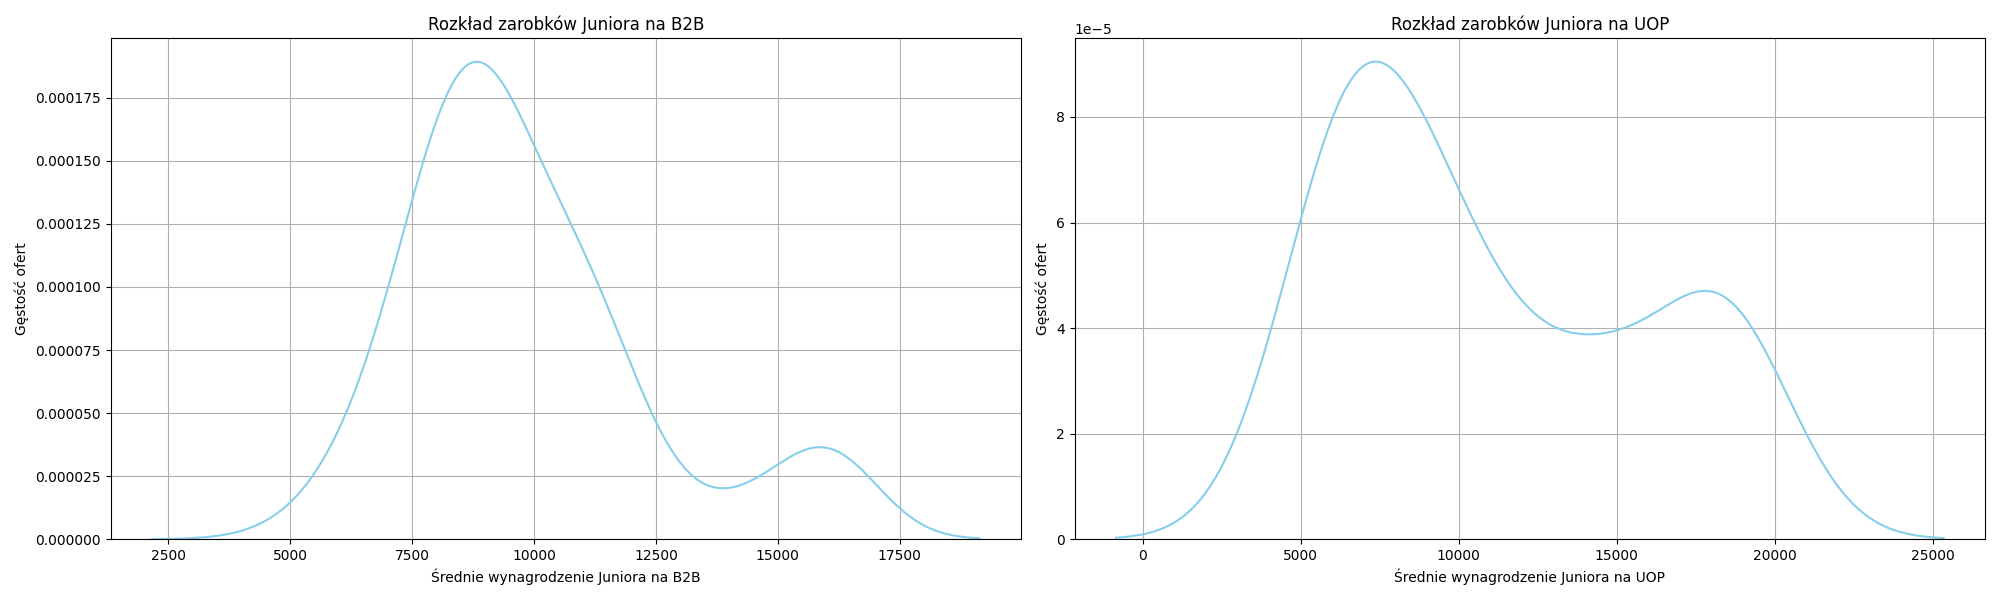
\includegraphics[width=0.8\textwidth]{../analysis/plots/rozkłady/pensje_dla_juniora.png}
    \caption{Rozkłady zarobków dla poszczególnych umów dla juniorów}
\end{figure}

\begin{figure}[H]
    \centering
    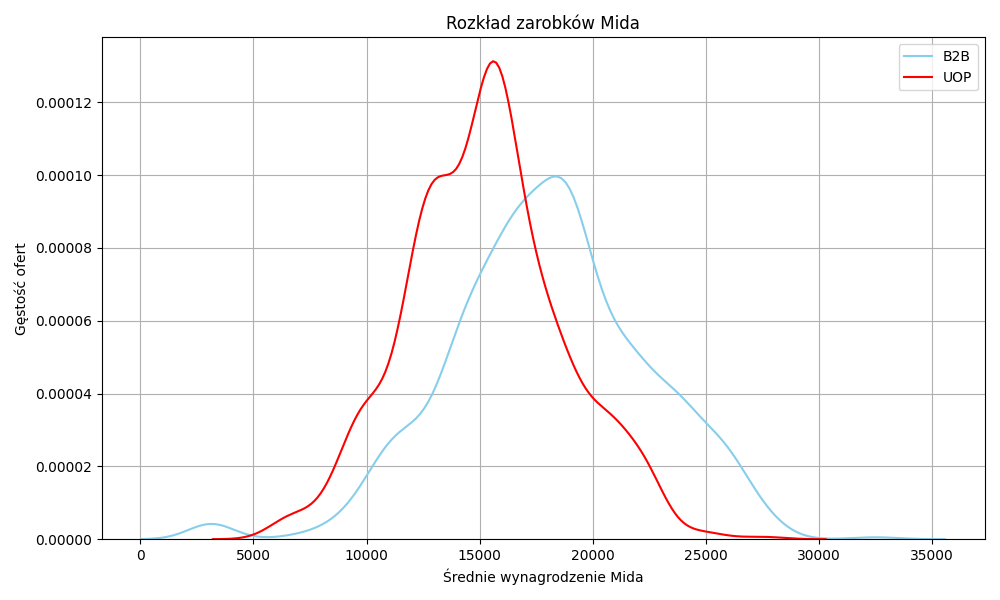
\includegraphics[width=0.8\textwidth]{../analysis/plots/rozkłady/pensje_dla_mida.png}
    \caption{Rozkłady zarobków dla poszczególnych umów dla midów}
\end{figure}

\begin{figure}[H]
    \centering
    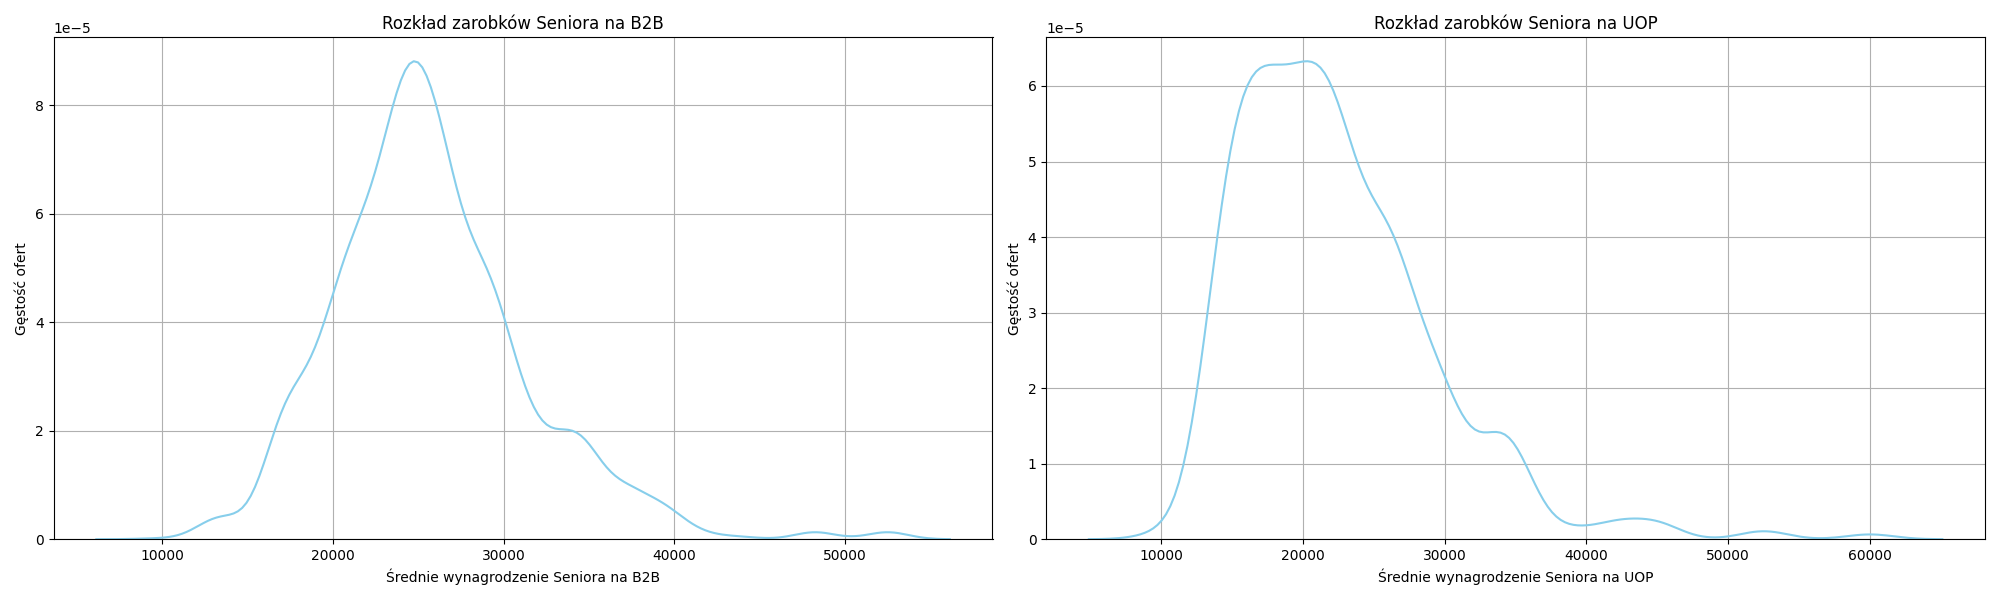
\includegraphics[width=0.8\textwidth]{../analysis/plots/rozkłady/pensje_dla_seniora.png}
    \caption{Rozkłady zarobków dla poszczególnych umów dla seniorów}
\end{figure}


\subsection{Jakie technologie są najbardziej poszukiwane?}

\begin{figure}[H]
    \centering
    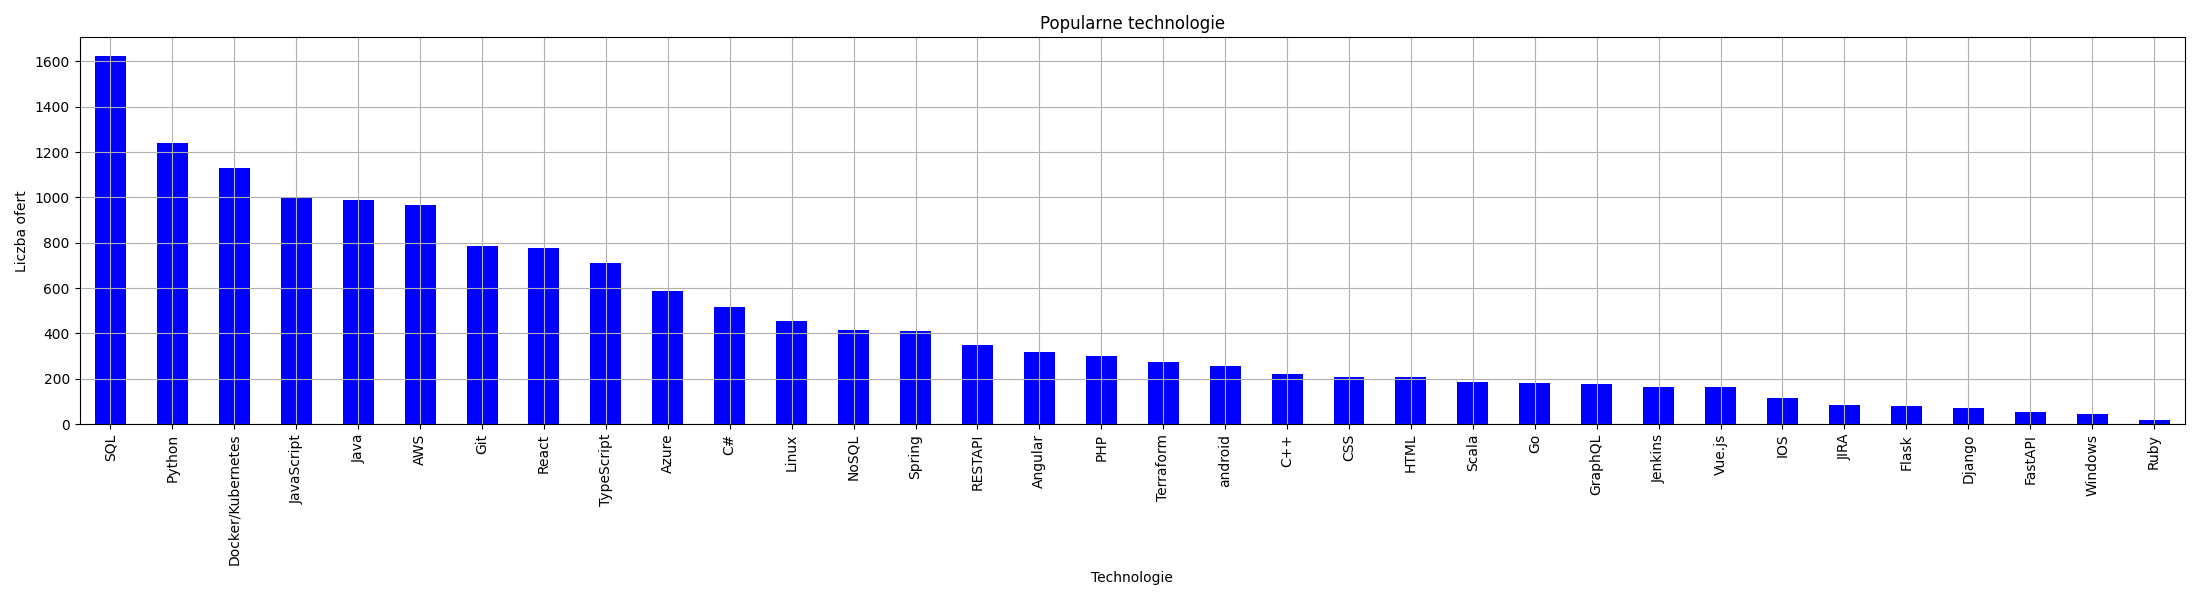
\includegraphics[width=\textwidth]{../analysis/plots/rozkłady/popularne_technologie.png}
    \caption{Popularne technologie w ofertach pracy w Polsce}
\end{figure}

\quad Tutaj moim zdaniem troche zaskoczenie ponieważ bez \texttt{SQL} ciężko znaleźć prace w IT, czyli
bazy danych to jest podstawa przy rekrutowanu się do pracy. Oczywiście nie mogło zabraknąć \texttt{Pythona} oraz \texttt{JavaScriptu} jeśli chodzi o języki skryptowe.
Co warto zazanczyć narzędzia takie jak \texttt{Docker} czy \texttt{Kubernetes} również są bardzo popularne i warto je znać. \texttt{Java} wygrywa z \texttt{C\#} a \texttt{GNU/Linux} deklasuje \texttt{Windowsa}.


\subsection{Gdzie jest największy popyt na programistów?}

\begin{figure}[H]
    \centering
    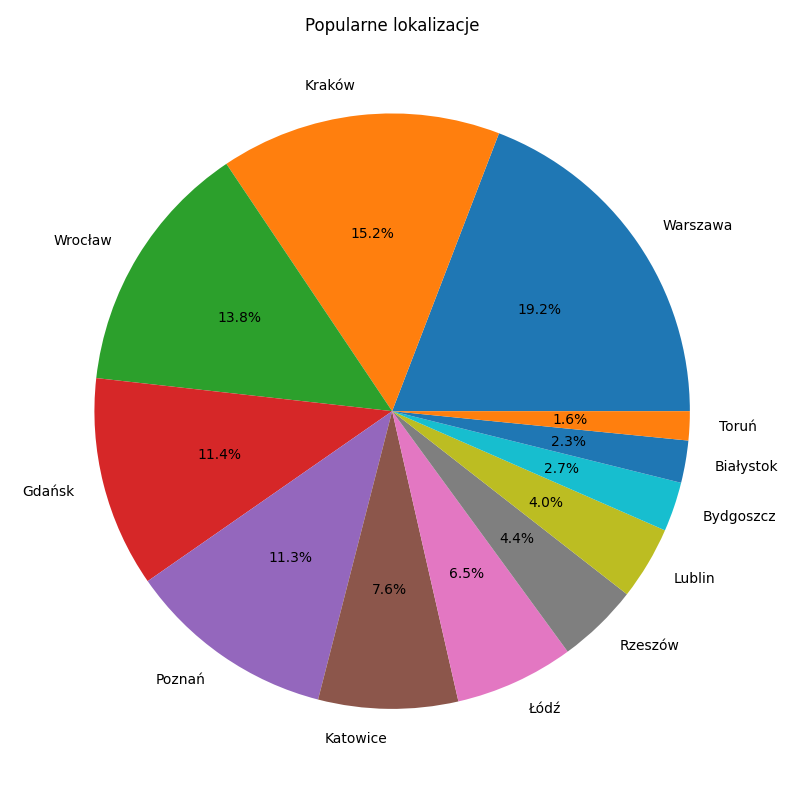
\includegraphics[width=0.8\textwidth]{../analysis/plots/rozkłady/popularne_lokalizacje.png}
    \caption{Popularne miasta w ofertach pracy w Polsce}
\end{figure}

\quad Zestawienie miast jest zgodne z oczekiwaniami, najwięcej ofert pracy jest kolejno w \textbf{Warszawie}, \textbf{Krakowie} oraz \textbf{Wrocławiu}, chociaż
\textbf{Gdańsk} również pojawiał się w dużej ilości ofert pracy.


\subsection{Gdzie poszukiwani są juniorzy?}

\begin{figure}[H]
    \centering
    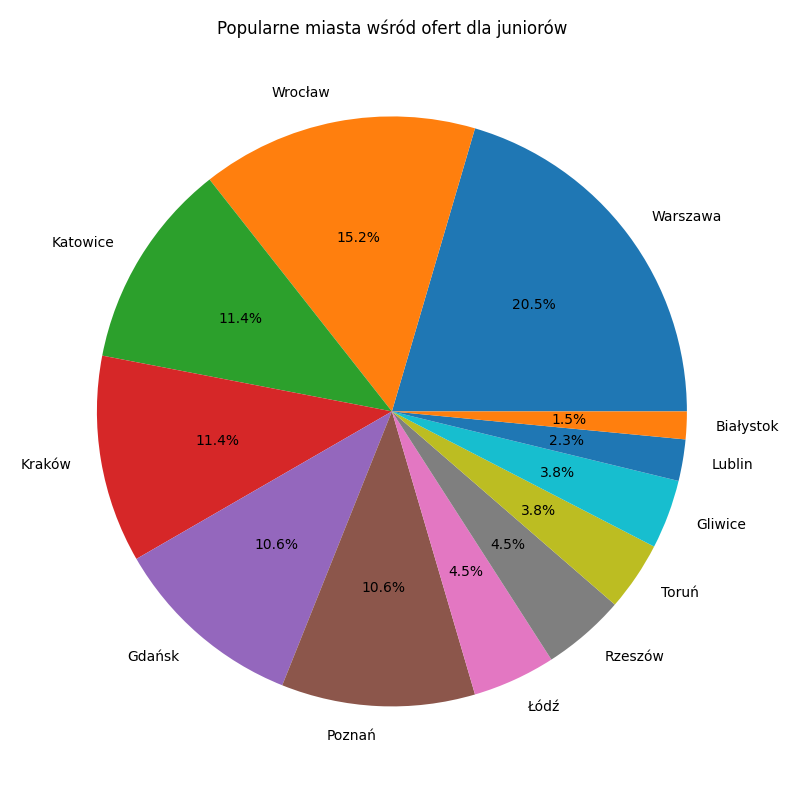
\includegraphics[width=\textwidth]{../analysis/plots/rozkłady/popularne_miasta_wśród_ofert_dla_juniorów.png}
    \caption{Popularne miasta w ofertach dla juniorów}
\end{figure}

\quad \textbf{Warszawa} jest najbardziej przyjazna dla juniorów, ale
warto zauważyć, że wykres nie różni się bardzo od poprzedniego z jednym, \textit{ale} - \textbf{Katowice} są
na 3 miejscu w zestawieniu dla juniorów, co może być zaskoczeniem.


\section{Powiązania między danymi}

\subsection{Powiązania między technologiami}

\begin{figure}[H]
    \centering
    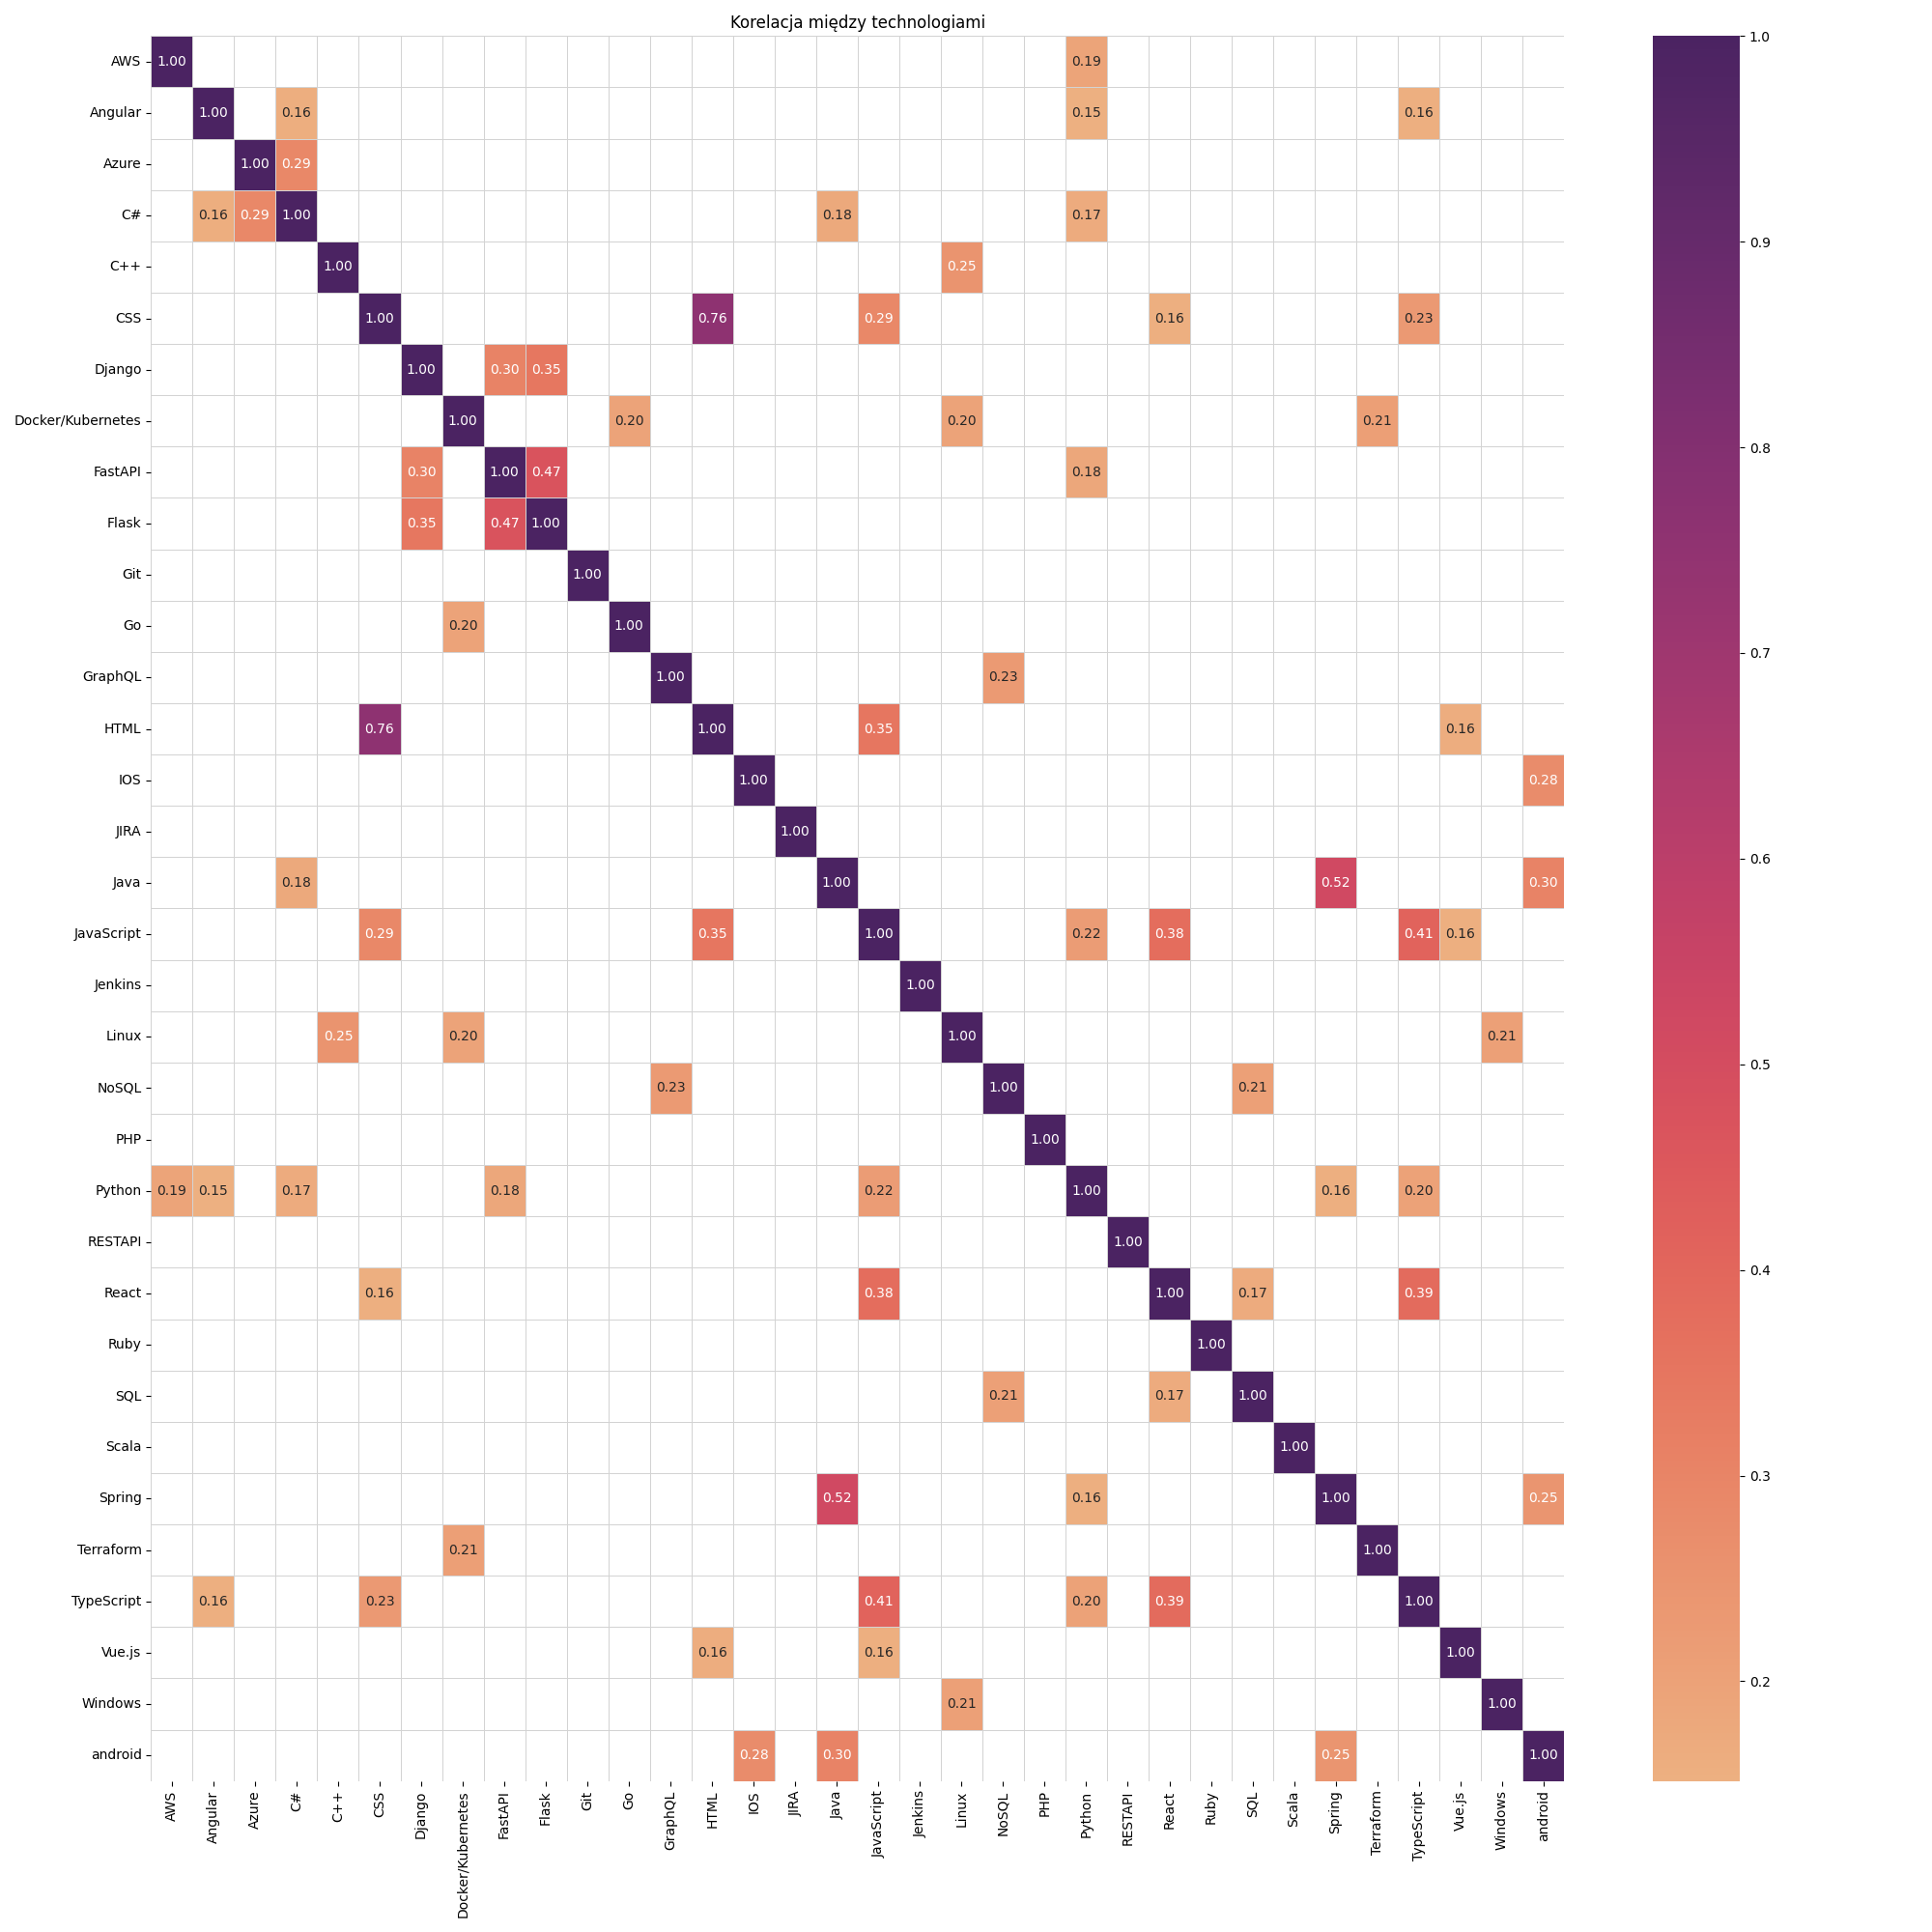
\includegraphics[width=\textwidth]{../analysis/plots/korelacje/korelacja_między_technologiami.png}
    \caption{Powiązania między technologiami, zawierająca tylko wartości korelacji większe niż 0.14}
\end{figure}

\quad \textbf{Co można zauważyć?}

\begin{enumerate}
    \item HTML i CSS idą ze prawie w parze - co jest zrozumiałe, bo to podstawy front-endu
    \item Przy Javie warto znać Springa
    \item React i JS i TS często pojawiają sie razem w ofertach pracy obok HTML i CSS
    \item Jak sie uczy Django to warto znać inne frameworki backendowe takie jak Flask czy FastAPI
    \item Jak sie idzie w Embedded to warto znać C/C++ oraz Linux
\end{enumerate}

\quad To tylko kilka przykładów wymienionych wynikający z obrazka powyżej, ale warto zauważyć, że nie ma tutaj dużo
powiązań między technologiami, co może wynikać z tego, że technologie są zbyt różne, aby były powiązane.


\subsection{Powiązania między innymi zmiennymi}

\begin{figure}[H]
    \centering
    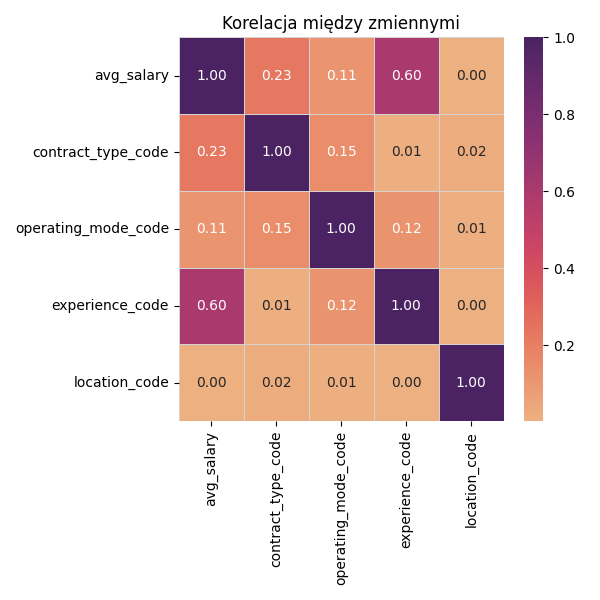
\includegraphics[width=\textwidth]{../analysis/plots/korelacje/korelacja_między_zmiennymi.png}
    \caption{Powiązania między innymi zmiennymi}
\end{figure}

\quad \textbf{Co można zauważyć?}

\begin{enumerate}
    \item W jakiś spobób powiązane są ze sobą zarobki na B2B i UOP - ma sens
    \item Wynagrodzenie na B2B i UOP jest powiązane z doświadczeniem
\end{enumerate}


\subsection{Zarobek a technologie}

\begin{figure}[H]
    \centering
    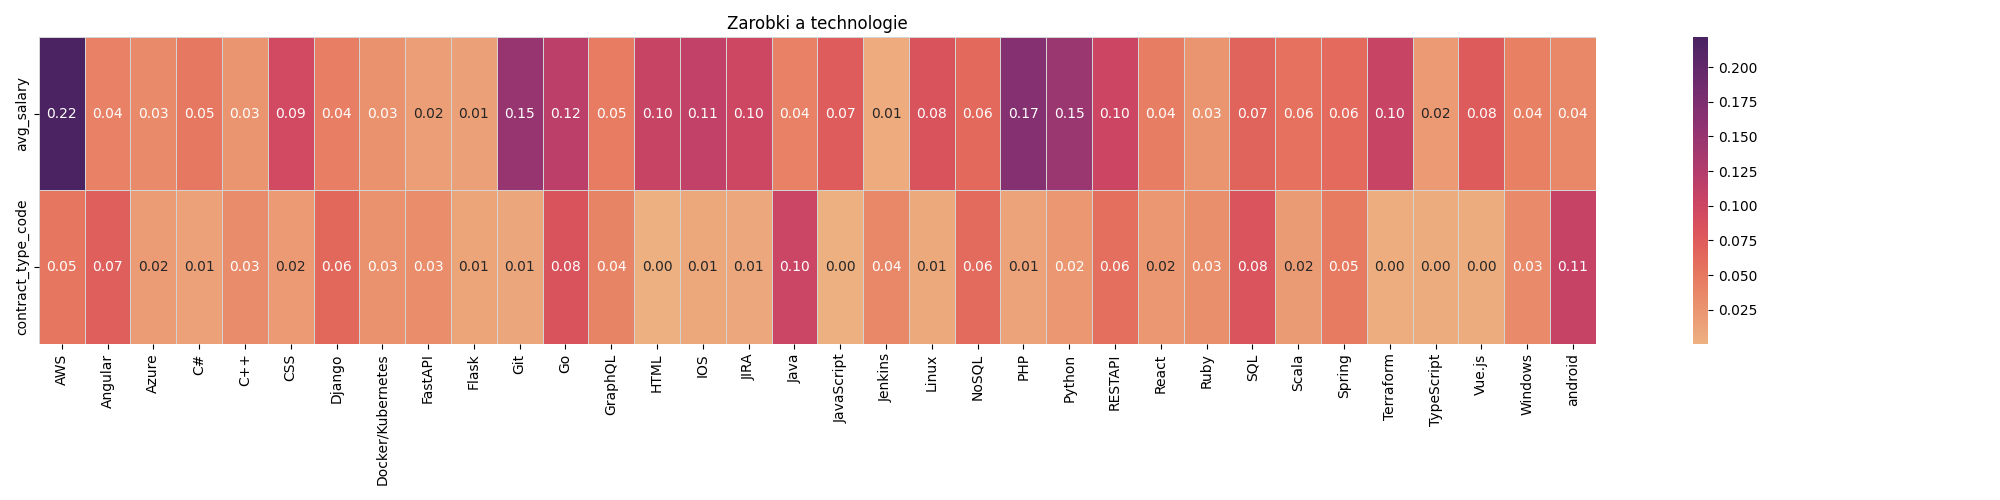
\includegraphics[width=\textwidth]{../analysis/plots/korelacje/zarobki_a_technologie.png}
    \caption{Powiązania między zarobkiem a technologiami}
\end{figure}

\quad Tutaj jest kilka ciekawych powiązań, które warto zauważyć, np. na umowie o prace znaczenie ma
znajomość: Go, AWS, Angulara, Java, SQL czy Andorida, chociaż nie są to mocne powiązania. Natomiast na B2B nie ma jakiś znaczących powiązań można wskazać
np. Resta, AWS, Docker/Kubernetes czy PHP, ale są to watości rzędu 0.09, co nie jest imponującym wynikiem.


\section{Czy da się przewidzieć zarobki, w zależności od mojego tech-stacku?}

\subsection{Ogólnie o problemie}

\quad \textbf{Oczywiście}, że tak, kiedy mamy dane to możemy nauczyć model, który na wejściu dostanie zmienne i przewidzi dla nas
zarobki. Dokładniej mówiąc model otrzyma na wejściu dane takie jak:

\texttt{Input:}

\begin{itemize}
    \item Tech-stack
\end{itemize}

\texttt{Output:}

\begin{itemize}
    \item Zarobki w PLN
\end{itemize}


\subsection{Dobór modeli}

\quad Modele które będą wykorzystane w analizie to:

\begin{enumerate}
    \item Regresja liniowa
          \begin{itemize}
              \item \texttt{LinearRegression}
              \item \texttt{Ridge}
              \item \texttt{Lasso}
              \item \texttt{ElasticNet}
          \end{itemize}
    \item \texttt{Decision tree}
    \item \texttt{Random forest}
\end{enumerate}

\textit{Wszyskie modele pochodzą z modułu \texttt{sklearn} dostępniej pod \href{https://scikit-learn.org/stable/}{tym linkiem}}

\subsection{Trochę statystyki - metryki}

\quad Do oceny modeli wykorzystam metryki takie jak:

\begin{itemize}
    \item \textbf{Mean Squared Error} - średni błąd kwadratowy
    \item \textbf{Root Mean Squared Error} - pierwiastek z średniego błędu kwadratowego
    \item \textbf{R-squared} - współczynnik determinacji $R^2$
    \item \textbf{Mean Absolute Error} - średni błąd bezwzględny
\end{itemize}

\subsubsection{Średni błąd kwadratowy}

\quad \textbf{Mean Squared Error (MSE)} - to metryka oceniająca jakość przewidywań modelu poprzez obliczenie średniego kwadratu różnicy między przewidywanymi a rzeczywistymi wartościami. Im niższa wartość MSE, tym lepiej model przewiduje rzeczywiste dane.

\begin{align}
    {MSE} ={\frac {1}{n}}\sum _{i=1}^{n}\left(Y_{i}-{\hat {Y_{i}}}\right)^{2}.
\end{align}

\subsubsection{Pierwiastek z średniego błędu kwadratowego}

\quad \textbf{Root Mean Squared Error (RMSE)} - to pierwiastek z MSE, co daje nam miarę błędu przewidywań w tych samych jednostkach co dane wejściowe. Jest bardziej intuicyjny w interpretacji niż MSE.

\subsubsection{Współczynnik determinacji}

\quad \textbf{R-squared (R2)} - to miara oceny dopasowania funkcji regresji do danych. Wartość bliska 1 oznacza, że funkcja regresji lepiej dopasowała sie do danych.

\begin{align} R^2&=1-\frac{\sum({y_i}-\hat{y_i})^2}{\sum(y_i-\bar{y})^2}, R^2 \in [0, 1] \end{align}

\subsubsection{Średni błąd bezwzględny}

\quad \textbf{Mean Absolute Error (MAE)} - to średni bezwzględny błąd między przewidywaniami a rzeczywistymi wartościami. MAE mierzy średnią wielkość błędów w przewidywaniach modelu, nie zwracając uwagi na kierunek błędu. Im niższa wartość MAE, tym lepiej model przewiduje rzeczywiste dane.

\begin{align}
    {\displaystyle \mathrm {MAE} ={\frac {\sum _{i=1}^{n}\left|y_{i}-x_{i}\right|}{n}}.}
\end{align}


\subsection{Wyniki oraz ograniczenia}

\quad Moje podejście opiera się na tworzeniu słownika modeli wraz z ich parametrami. Na samym początku,
jeszcze przed wyborem konkretnego modelu, dokonuję doboru optymalnych parametrów dla
każdego z nich. Tutaj można to zrobić na dwa sposoby, ręcznie lub za pomocą \texttt{GridSearchCV} z \texttt{sklearn}.
W moim przypadku dobrałem ręcznie parametry, ponieważ po tuningu parametrów modelowi brakowało danych (?), i algorytm
zwracał błąd.

\quad Kolejnym krokiem jest przeprowadzenie procesu uczenia modelu na dostępnych
danych. Po zakończeniu tego etapu prezentuję wyniki metryk dla najlepszego modelu i zwracam już
wytrenowany model. Następnie udostępniam możliwość przewidywania zarobków dla większego zbioru danych.

\textbf{Ograniczenia} - tutaj warto zauważyć jedną rzecz, dla niektórych tech-stacków model nie jest w stanie
przewidzieć zarobków, ponieważ nie ma tak dużo danych w zbiorze. W tym przypadku można bybyło rozszerzyć zbiór
danych o kolejne ofert - zautomatyzować proces pobierania danych, czyli aktualizować bazę co klika dni.

\textbf{Wyniki} - zwracane modele mogą się różnić w zależności od danych wejściowych, czyli np.
dla Java, Spring może zostać wybrany model \texttt{Ridge} a dla Pythona wybrany może być \texttt{RandomForest}, no i oczywiście zwrócony
model jest już wytrenowany na danych, które zostały podane na wejściu, więc przy ponownym przewidzeniu zarobków dajemy
mu tylko więcej danych. Na koniec tworze wizuazlizację wyników, gdzie mamy porównanie rzeczywistych zarobków z przewidywanymi.

\begin{abstract}
    \textbf{Proponowane tech-stacki do uczenia}
    \quad Na tych poszczególnych technologiach będą się uczyć modele, a następnie zostanie wybrany najlepszy
    \begin{itemize}
        \item Python
        \item JavaScript, React
        \item Docker/Kubernetes, AWS
    \end{itemize}

    \textbf{Pozostałe dane do wyznaczenie zarobków dla powyższych tech-stacków oraz innych zmiennych:}
    \begin{table}[H]
        \centering
        \begin{tabular}{|l|l|l|l|}
            \hline
            \textbf{Tech-stacki}   & \textbf{Lokalizacja} & \textbf{Doświadczenie} & \textbf{Typ kontraktu} \\ \hline
            Python                 & Warszawa             & Junior                 & B2B                    \\ \hline
            JavaScript, React      & Kraków               & Mid                    & UOP                    \\ \hline
            Docker/Kubernetes, AWS & Wrocław              & Senior                 & B2B                    \\ \hline
        \end{tabular}
    \end{table}

\end{abstract}

\subsubsection{Wyniki dla podziału danych 80:20}
\quad Analizę wyników przeprowadzę dla podziału danych 80:20, gdzie 80\% danych to dane treningowe, a 20\% to dane testowe.


\textbf{Co z tego wynika?}

\quad Model będzie miał wystarczająco dużo danych do nauki w przypadku popularnych technologii, zatem
dane, które będziemy przewidywać będą lepiej dopasowane w teorii.

\begin{table}[H]
    \centering
    \begin{tabular}{|l|l|l|l|l|}
        \hline
        \textbf{Modele}                         & \textbf{MSE} & \textbf{MAE} & \textbf{RMSE} & \textbf{R2} \\ \hline
        LinearRegression()                      & 28422749.87  & 4358.93      & 5331.30       & 0.4238      \\ \hline
        DecisionTreeRegressor()                 & 28263018.93  & 4312.16      & 5316.30       & 0.4271      \\ \hline
        RandomForestRegressor(n\_estimators=20) & 28284532.84  & 4330.01      & 5318.32       & 0.4266      \\ \hline
        Ridge(alpha=0.1)                        & 28422322.40  & 2918.68      & 5331.26       & 0.4238      \\ \hline
        Lasso()                                 & 28422009.47  & 4358.85      & 5331.30       & 0.4238      \\ \hline
    \end{tabular}
\end{table}


Wybrany model to DecisionTreeRegressor(), ponieważ ma największy współczynnik determinacji $R^2$.
Przewidywane zarobki dla Juniora znającego ['Python'] w lokalizacji Warszawa na umowie b2b to: \textbf{9400.0 PLN}.

\begin{figure}[H]
    \centering
    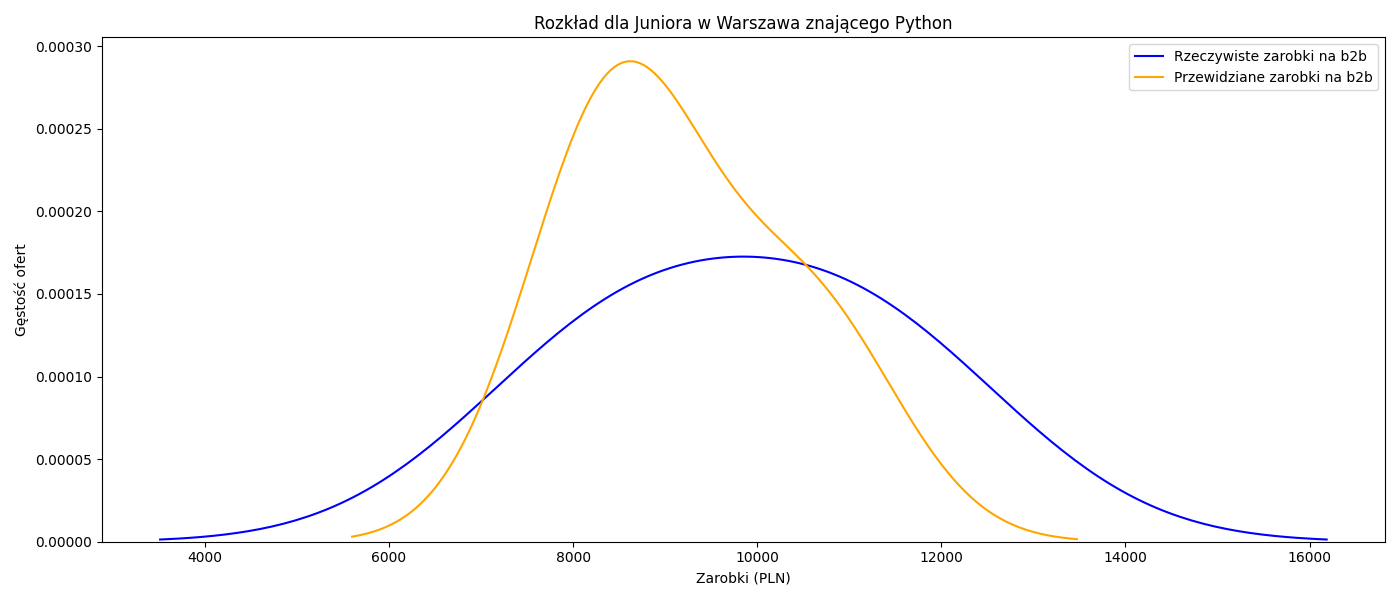
\includegraphics[width=\textwidth]{../analysis/plots/wyniki/0.8&0.2/przewidywane_zarobki_dla_juniora_w_warszawa_Python.png}
\end{figure}


\begin{table}[H]
    \centering
    \begin{tabular}{|l|l|l|l|l|}
        \hline
        \textbf{Modele}                         & \textbf{MSE} & \textbf{MAE} & \textbf{RMSE} & \textbf{R2} \\ \hline
        LinearRegression()                      & 13221438.39  & 2919.54      & 3636.13       & 0.4823      \\ \hline
        DecisionTreeRegressor()                 & 21276698.63  & 3431.44      & 4612.67       & 0.1669      \\ \hline
        RandomForestRegressor(n\_estimators=20) & 18433724.47  & 3192.39      & 4293.45       & 0.2782      \\ \hline
        Ridge(alpha=0.1)                        & 13213875.66  & 2918.68      & 3635.09       & 0.4826      \\ \hline
        Lasso()                                 & 13219274.21  & 2919.21      & 3635.83       & 0.4824      \\ \hline
    \end{tabular}
\end{table}


Wybrany model to \texttt{Ridge} z wartością \texttt{alpha=0.1}, ponieważ ma najniższe wartości błędów oraz najwyższy współczynnik determinacji $R^2$.
Przewidywane zarobki dla Mida znającego ['JavaScript', 'React'] w lokalizacji Kraków na umowie uop to: \textbf{15028.69 PLN}.
\begin{figure}[H]
    \centering
    \includegraphics[width=\textwidth]{../analysis/plots/wyniki/0.8&0.2/przewidywane_zarobki_dla_mida_w_kraków_JavaScript_React.png}
    \caption{Przewidywane zarobki dla mida znającego JS i React w Krakowie na uop}
\end{figure}


\begin{table}[H]
    \centering
    \begin{tabular}{|l|l|l|l|l|}
        \hline
        \textbf{Modele}                         & \textbf{MSE} & \textbf{MAE} & \textbf{RMSE} & \textbf{R2} \\ \hline
        LinearRegression()                      & 11084299.37  & 2678.04      & 3329.31       & 0.6751      \\ \hline
        DecisionTreeRegressor()                 & 10681171.68  & 2605.54      & 3268.21       & 0.6870      \\ \hline
        RandomForestRegressor(n\_estimators=20) & 10691260.30  & 2643.63      & 3269.75       & 0.6867      \\ \hline
        Ridge(alpha=0.1)                        & 11091505.44  & 2678.65      & 3330.39       & 0.6749      \\ \hline
        Lasso()                                 & 11085643.78  & 2678.07      & 3329.51       & 0.6751      \\ \hline
    \end{tabular}
\end{table}


Wybrany model to \texttt{DecisionTreeRegressor}, ponieważ ma najniższe wartości błędów oraz najwyższy współczynnik determinacji $R^2$.
Przewidywane zarobki dla Seniora znającego ['Docker/Kubernetes', 'AWS'] w lokalizacji Wrocław na umowie b2b to: \textbf{27391.62 PLN}.
\begin{figure}[H]
    \centering
    \includegraphics[width=\textwidth]{../analysis/plots/wyniki/0.8&0.2/przewidywane_zarobki_dla_seniora_w_wrocław_Docker_Kubernetes_AWS.png}
    \caption{Przewidywane zarobki dla seniora w Wrocławiu znającego Docker, Kubernetes oraz AWS na b2b}
\end{figure}



\subsubsection{Wyniki dla podziału danych 60:40}

\begin{table}[H]
    \centering
    \begin{tabular}{|l|l|l|l|l|}
        \hline
        \textbf{Modele}                         & \textbf{MSE} & \textbf{MAE} & \textbf{RMSE} & \textbf{R2} \\ \hline
        LinearRegression()                      & 29050483.53  & 4406.48      & 5389.85       & 0.4097      \\ \hline
        DecisionTreeRegressor()                 & 29520117.74  & 4434.43      & 5433.24       & 0.4001      \\ \hline
        RandomForestRegressor(n\_estimators=20) & 29210648.93  & 4417.47      & 5404.67       & 0.4064      \\ \hline
        Ridge(alpha=0.1)                        & 29050015.21  & 4406.39      & 5389.81       & 0.4097      \\ \hline
        Lasso()                                 & 29049387.82  & 4406.36      & 5389.75       & 0.4238      \\ \hline
    \end{tabular}
\end{table}


Wybrany model to \texttt{Lasso}, ponieważ ma największy współczynnik determinacji $R^2$.
Przewidywane zarobki dla Juniora znającego ['Python'] w lokalizacji Warszawa na umowie b2b to: \textbf{9398.07 PLN}.

\begin{figure}[H]
    \centering
    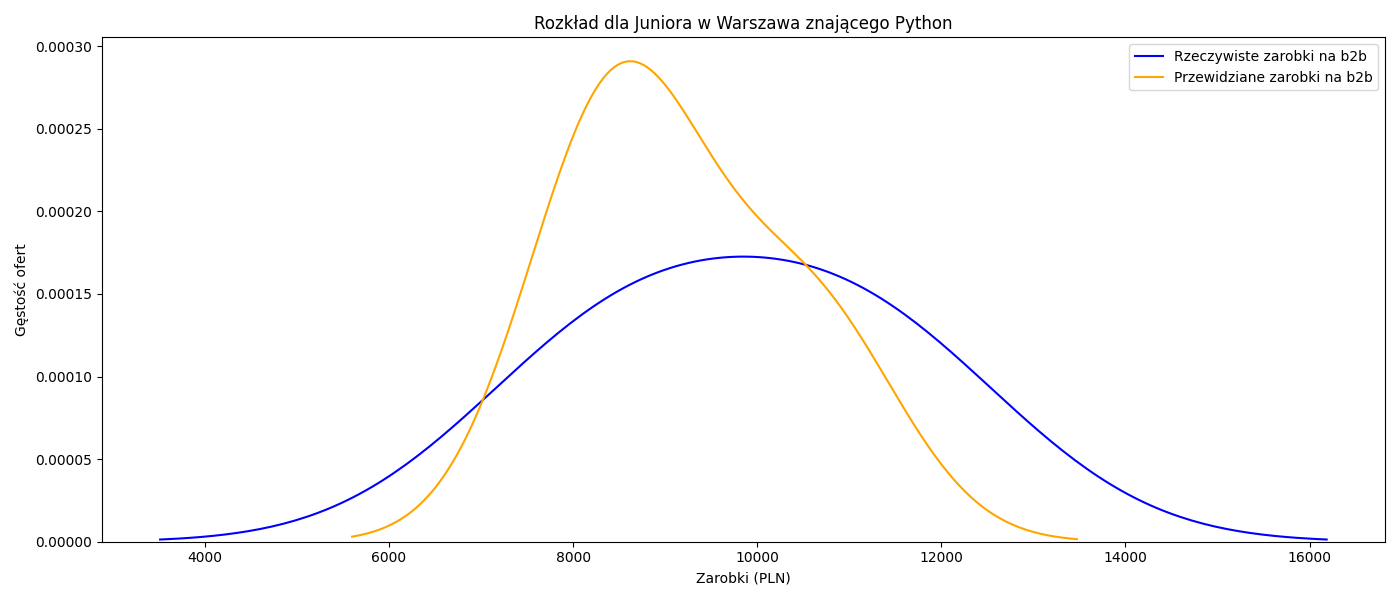
\includegraphics[width=\textwidth]{../analysis/plots/wyniki/0.8&0.2/przewidywane_zarobki_dla_juniora_w_warszawa_Python.png}
\end{figure}


\begin{table}[H]
    \centering
    \begin{tabular}{|l|l|l|l|l|}
        \hline
        \textbf{Modele}                         & \textbf{MSE} & \textbf{MAE} & \textbf{RMSE} & \textbf{R2} \\ \hline
        LinearRegression()                      & 17512382.62  & 3014.49      & 4184.78       & 0.4212      \\ \hline
        DecisionTreeRegressor()                 & 21206971.44  & 3442.39      & 4605.10       & 0.2991      \\ \hline
        RandomForestRegressor(n\_estimators=20) & 18610952.15  & 3251.63      & 4314.04       & 0.3849      \\ \hline
        Ridge(alpha=0.1)                        & 17503667.86  & 3014.10      & 4183.74       & 0.4215      \\ \hline
        Lasso()                                 & 17512097.61  & 3014.5       & 4184.74       & 0.4212      \\ \hline
    \end{tabular}
\end{table}


Wybrany model to \texttt{Ridge} z wartością \texttt{alpha=0.1}, ponieważ ma najniższe wartości błędów oraz najwyższy współczynnik determinacji $R^2$.
Przewidywane zarobki dla Mida znającego ['JavaScript', 'React'] w lokalizacji Kraków na umowie uop to: \textbf{14872.58 PLN}.


\begin{figure}[H]
    \centering
    \includegraphics[width=\textwidth]{../analysis/plots/wyniki/0.8&0.2/przewidywane_zarobki_dla_mida_w_kraków_JavaScript_React.png}
    \caption{Przewidywane zarobki dla mida znającego JS w React w Krakowie na uop}
\end{figure}


\begin{table}[H]
    \centering
    \begin{tabular}{|l|l|l|l|l|}
        \hline
        \textbf{Modele}                         & \textbf{MSE} & \textbf{MAE} & \textbf{RMSE} & \textbf{R2} \\ \hline
        LinearRegression()                      & 10035694.55  & 2466.69      & 3167.92       & 0.70586     \\ \hline
        DecisionTreeRegressor()                 & 10593012.16  & 2564.23      & 3254.69       & 0.68953     \\ \hline
        RandomForestRegressor(n\_estimators=20) & 10042038.81  & 2513.25      & 3168.917      & 0.70568     \\ \hline
        Ridge(alpha=0.1)                        & 10036240.1   & 2467.61      & 3168.002      & 0.70585     \\ \hline
        Lasso()                                 & 10036562.26  & 2466.89      & 3168.053      & 0.70584     \\ \hline
    \end{tabular}
\end{table}


Wybrany model to \texttt{LinearRegression}, ponieważ ma najniższe wartości błędów oraz najwyższy współczynnik determinacji $R^2$.
Przewidywane zarobki dla Seniora znającego ['Docker/Kubernetes', 'AWS'] w lokalizacji Wrocław na umowie b2b to: \textbf{28221.87 PLN.}
\begin{figure}[H]
    \centering
    \includegraphics[width=\textwidth]{../analysis/plots/wyniki/0.8&0.2/przewidywane_zarobki_dla_seniora_w_wrocław_Docker_Kubernetes_AWS.png}
    \caption{Przewidywane zarobki dla seniora w Wrocławiu znającego Docker, Kubernetes oraz AWS na b2b}
\end{figure}

\newpage

\subsection{Wnioski}

\quad Co do podziału 80/20 oraz 60/40 to wyniki są bardzo podobne, ale warto zauważyć, że dla podziału 60/40 zarobki są niższe - bardziej realne.
Warto zauważyć, najlepsze modele zależą od teck-stacku, ale najczęsciej wyberany był model \texttt{Ridge}.
Klasyczny model regresji liniowej pojawił się raz gdy mieliśmy określoną jedną technologię i była ona bardzo częsta w ofertach, czyli
musi dla bardziej rozwiniętej bazy prawdopodobnie ten model byłby całkiem dobry. Warto dodać błędy \texttt{MAE} oraz \texttt{RMSE} są na poziomie kilku tysięcy PLN
co jest dobrym wynikiem dla ofert skierowanych dla midów, a zwłaszcza dla seniorów, gorzej jest z juniorami, ponieważ błędy są duże jak na przewidzianą pensję,
wynika to z tego, że obecnie na rynku jest relatywnie mało ofert dla tej grupy. Ostatnią rzeczą może być to, że współczynnik determinacji $R^2$ jest ogólnie całkiem wysoki,
chociaż on wynika z tego, że ogólnie danych treningowych było sporo, gorzej może być w przypadku gdybyśmy chcieli przewidzieć niszowe technologie np. Ruby z C++.
Ogónie można powiedzieć, że wyniki są trochę zawyżone co może wynikać z tego, że w ofertach pojawiały się
bardzo duże zarobki, które mogą być wyjątkiem, a nie regułą.

\quad Koniec końców, nie udało się wyuczyć jednego modelu, ale udało się stworzyć algorytm dobierający odpowiedni model do danych wejściowych.
Warto dodać, że projekt może być udoskonalony o algorytm, który będzie automatyzować proces pobierania danych, czyli aktualizować bazę co klika dni,
mogło by to wzbogacić bazę danych o nowe oferty pracy, a co za tym idzie poprawić wyniki modeli.
\end{document}


